\begin{table}[H]\centering\small
\caption{Полное время запуска}
\begin{tabular}{rlrrr}\toprule
Длина & Раннер & Медиана, мс & $Q_1$ & $Q_3$\\\midrule
100 & Jest & 1011.1 & 984.3 & 1082.0\\
100 & Mocha & 641.0 & 610.4 & 657.7\\
100 & Vitest & 1176.2 & 1156.5 & 1199.5\\
1000 & Jest & 1072.4 & 1051.6 & 1120.8\\
1000 & Mocha & 635.9 & 623.0 & 644.8\\
1000 & Vitest & 1182.2 & 1175.4 & 1220.4\\
10000 & Jest & 1577.1 & 1554.0 & 1647.0\\
10000 & Mocha & 690.4 & 675.6 & 710.2\\
10000 & Vitest & 1228.9 & 1222.9 & 1253.8\\
\bottomrule\end{tabular}\end{table}

\begin{table}[H]\centering\small
\caption{Накопленное CPU-время, нижняя оценка}
\begin{tabular}{rlrrr}\toprule
Длина & Раннер & Медиана, мс & $Q_1$ & $Q_3$\\\midrule
100 & Jest & 1078.1 & 1054.7 & 1210.9\\
100 & Mocha & 578.1 & 515.6 & 640.6\\
100 & Vitest & 1234.4 & 1179.7 & 1328.1\\
1000 & Jest & 1218.8 & 1164.1 & 1234.4\\
1000 & Mocha & 578.1 & 562.5 & 609.4\\
1000 & Vitest & 1234.4 & 1195.3 & 1296.9\\
10000 & Jest & 1781.2 & 1687.5 & 1796.9\\
10000 & Mocha & 656.2 & 609.4 & 710.9\\
10000 & Vitest & 1343.8 & 1281.2 & 1382.8\\
\bottomrule\end{tabular}\end{table}

\begin{table}[H]\centering\small
\caption{Наблюдаемый пик суммы RSS}
\begin{tabular}{rlrrr}\toprule
Длина & Раннер & Медиана, MiB & $Q_1$ & $Q_3$\\\midrule
100 & Jest & 146.7 & 146.3 & 146.7\\
100 & Mocha & 103.6 & 103.4 & 103.9\\
100 & Vitest & 177.4 & 177.3 & 177.8\\
1000 & Jest & 146.9 & 146.7 & 147.3\\
1000 & Mocha & 103.5 & 103.4 & 103.7\\
1000 & Vitest & 178.0 & 177.8 & 178.4\\
10000 & Jest & 146.3 & 146.1 & 146.7\\
10000 & Mocha & 103.8 & 103.7 & 105.3\\
10000 & Vitest & 177.8 & 177.6 & 177.9\\
\bottomrule\end{tabular}\end{table}

\begin{figure}[H]\centering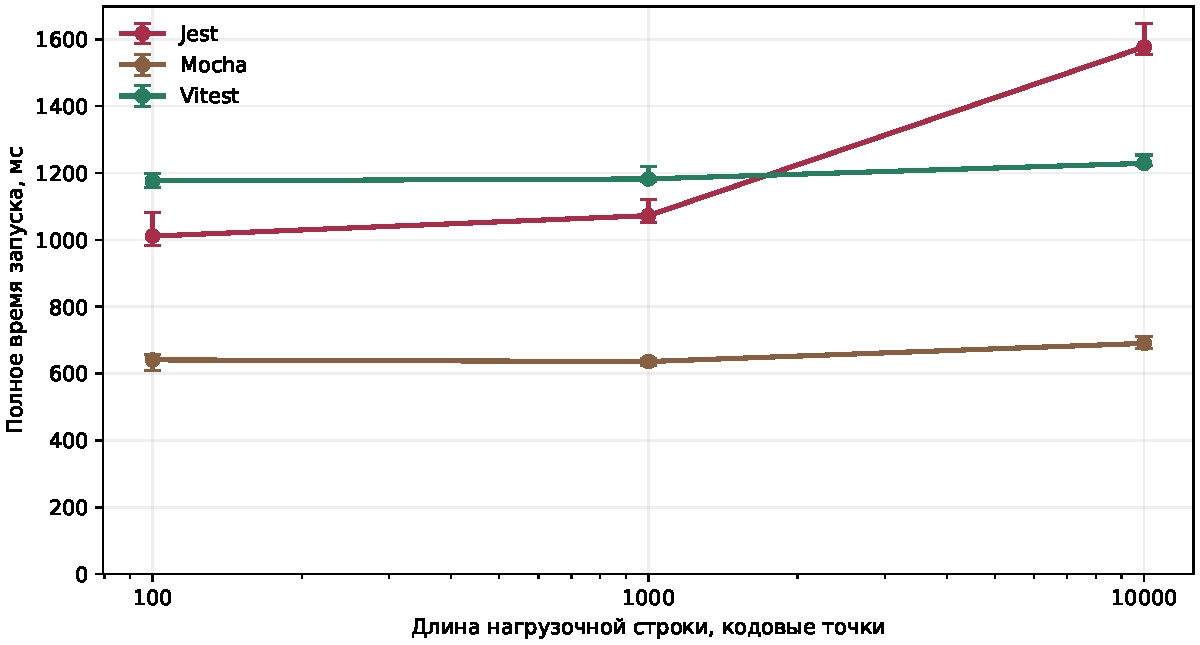
\includegraphics[width=.94\linewidth]{report/time.pdf}\caption{Полное время запуска. Точки -- медианы, отрезки -- первый и третий квартили.}\end{figure}

\begin{figure}[H]\centering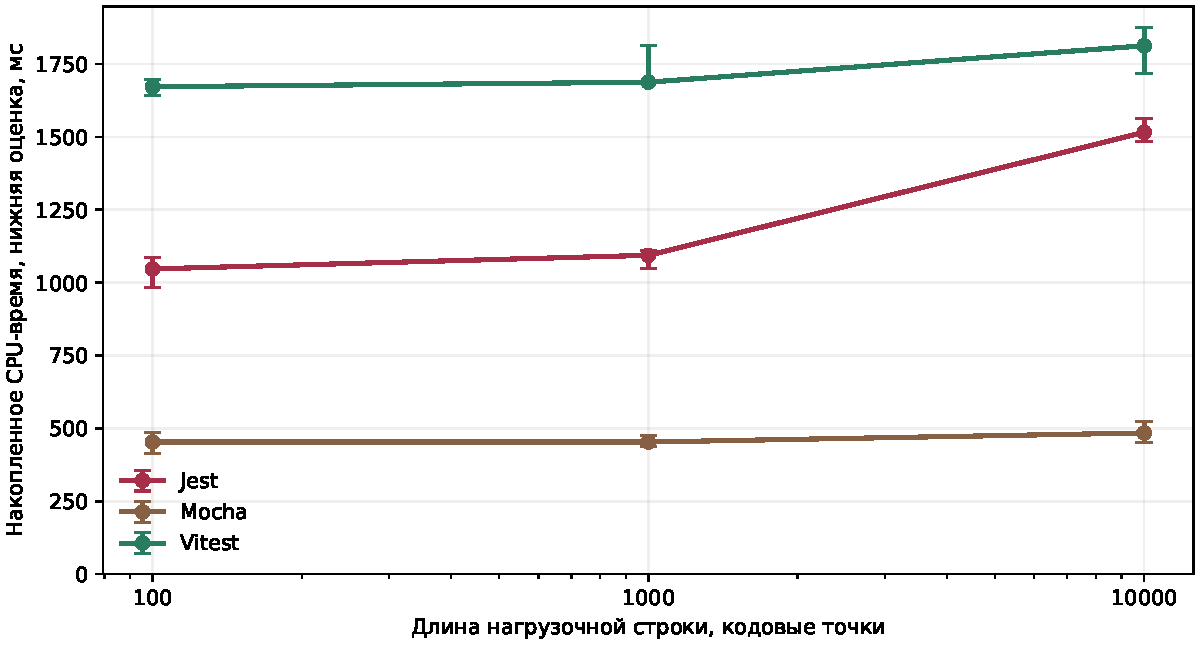
\includegraphics[width=.94\linewidth]{report/cpu.pdf}\caption{Накопленное CPU-время, нижняя оценка. Точки -- медианы, отрезки -- первый и третий квартили.}\end{figure}

\begin{figure}[H]\centering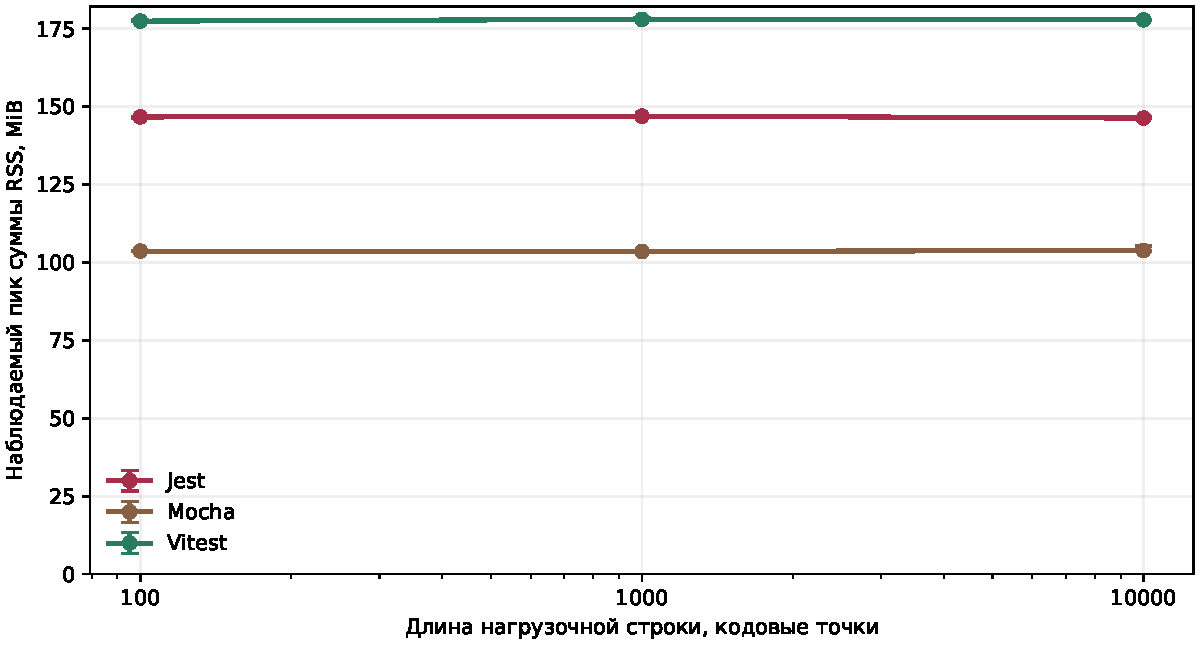
\includegraphics[width=.94\linewidth]{report/memory.pdf}\caption{Наблюдаемый пик суммы RSS. Точки -- медианы, отрезки -- первый и третий квартили.}\end{figure}

\begin{table}[H]\centering\small
\caption{Средняя CPU-загрузка в единицах одного логического процессора}
\begin{tabular}{rlrrr}\toprule
Длина & Раннер & Медиана, \% & $Q_1$ & $Q_3$\\\midrule
100 & Jest & 105.5 & 103.6 & 116.6\\
100 & Mocha & 88.5 & 84.2 & 101.1\\
100 & Vitest & 108.3 & 101.0 & 109.8\\
1000 & Jest & 110.7 & 105.3 & 115.4\\
1000 & Mocha & 90.9 & 87.9 & 95.6\\
1000 & Vitest & 104.4 & 100.3 & 108.1\\
10000 & Jest & 112.9 & 100.0 & 114.4\\
10000 & Mocha & 96.4 & 90.0 & 100.2\\
10000 & Vitest & 105.8 & 105.1 & 109.6\\
\bottomrule\end{tabular}\end{table}

В каждом запуске пройдены 99 тестов. Минимальное число отсчётов равно 41; максимальный интервал между обходами -- 30.6 мс. Обнаружено от 9 до 14 процессов на запуск. Различие числа обнаруженных процессов также может отражать пропуск коротких процессов при опросе.
